\begin{frame}
 \frametitle{Computational Complexity}
 \begin{itemize}
  \item Given
   \begin{itemize}
    \item Algorithm
    \item Input of length \( n \)
   \end{itemize}
  \item How many steps are necessary to complete algorithm as \( n \rightarrow \infty \)?
 \end{itemize}
 \begin{itemize}
  \item Big-O notation
  \item \( algorithm(n) = O(steps(n)) \) as \(n \rightarrow \infty \)
 \end{itemize}
\end{frame}

\begin{frame}
 \frametitle{Typical Complexity Classes}
 \begin{description}
  \item[\(O(1)\)] constant complexity, sign function, absolute values, searching in well-tuned hash tables
  \item[\(O(logn)\)] logarithmic complexity, binary searches, balanced search trees
  \item[\(O(n)\)] linear complexity, linear searching
  \item[\(O(nlogn)\)] linearithmic complexity, building search trees \\ \hfill \\
  \item[\(O(n^k)\)] polynomial complexity, naive sorting (e.g, bubble sort), matrix multiplication \\ \hfill \\
  \item[\(O(k^n)\)] exponential complexity, traveling salesman problem
 \end{description}
 \begin{itemize}
  \item example \filename{sort.c}
 \end{itemize}
\end{frame}

\begin{frame}
 \frametitle{Typical Complexity Classes}
 \begin{figure}
  \centering{
   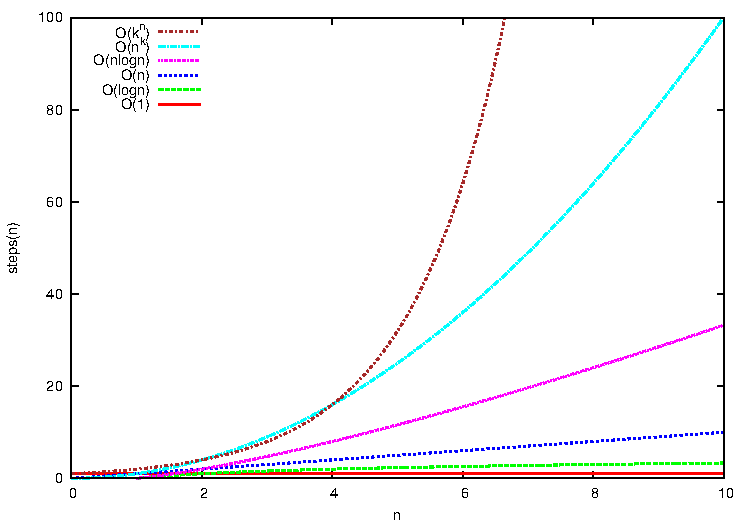
\includegraphics[scale=0.75]{complexity-gpi.pdf}
  }
  \caption{Complexity Classes}
 \end{figure}
\end{frame}

\begin{frame}
 \frametitle{Determining Complexity}
 \begin{itemize}
  \item use standard algorithms with known complexity
 \end{itemize}

 \centering{or}

 \begin{itemize}
  \item try to describe relation between \( n \) and number of primitive operations
  \item example of bubble sort
  \begin{enumerate}
   \item \(n\) iterations
   \item first iteration: \( n-1 \) compare operations
   \item second iteration: \( n-2 \) compare operations
   \item \(n'th\) iteration: \( n-n = 0 \) compare operations
   \item average per iteration: \( n/2 \) compare operations
   \item overall complexity: \( O(n * n/2) = O(n^2 / 2) = O(n^2) \)
  \end{enumerate}
  \item combinations of algorithms have the maximum complexity of primitive algorithms
  \item example of bubble-sorting absolute values
  \begin{enumerate}
   \item walk over all elements (\( O(n) \))
   \begin{itemize}
    \item compute absolute value for each element (\( O(1) \))
   \end{itemize}
   \item bubble-sort the results (\( O(n^2) \))
   \item overall complexity: \( O(n*1 + n^2) = O(n^2) \)
  \end{enumerate}
 \end{itemize}
\end{frame}

\begin{frame}
 \frametitle{Which Algorithm Is Best?}
 \begin{itemize}
  \item naive answer: use algorithm with lowest complexity
  \item but there are exceptions
  \begin{itemize}
   \item \(n\) is small
   \item better algorithms come with setup costs (e.g., binary searches need sorted input)
   \item hardware has branch prediction and is optimized for linear memory access (by prefetching memory)
   \begin{itemize}
    \item binary searches hop around in elements
    \item linear searches will walk over elements
   \end{itemize}
  \end{itemize}
  \item also consider other resources
 \end{itemize}
 \begin{itemize}
  \item \book{B. Kernighan, R. Pike}{The Practice of Programming}{Addison-Wesley 1999}
 \end{itemize}
\end{frame}
